\chapter{Teoretická část}
\section{Digitální dvojčata a územní plánování}
\section{Rozšířená realita}
Rozšířená realita je technologie, která v reálném čase spojuje fyzický svět s digitálními prvky, a to jak v trojrozměrné, tak ve dvourozměrné podobě. Umožňuje uživatelům interagovat s těmito digitálními objekty pomocí několika metod ovládání, jako jsou např. pohyb zařízení, dotykové ovládání nebo hlasové příkazy. \cite{AROverview}
\subsection{Klíčové aspekty}
Stejně jako každá technologie, i rozšířená realita má své klíčové aspekty, které jsou nezbytné pro její správné fungování.
\subsubsection{Snímání reality}
Snímání reality, kdy kamery a senzory zachycují reálné prostředí a detekují klíčové body a plochy v prostoru, což umožňuje správné zobrazení a interakci digitálních objektů s fyzickým prostředím jako takovým. \cite{AROverview}
\subsubsection{Pozicování}
Pozicování, které zajišťuje přesné určení pozice zařízení v prostoru. Rozšířená realita také využívá různé senzory, jako jsou GPS, akcelerometry nebo gyroskopy, k určení orientace a pozice zařízení. Díky kombinaci těchto senzorů dokáže zařízení rozšířené reality rozeznat pohyb, orientaci a pozici, což je nezbytné pro správné umístění a zobrazení digitálních objektů. \cite{AROverview}
\subsubsection{Vykreslování}
Vykreslování poskytuje realistické zobrazení digitálních objektů v souladu s perspektivou a měřítkem. Digitální objekty se tak zobrazují v přesné poloze a vypadají, jako by byly přímou součástí reálného světa. \cite{AROverview} \\
\subsection{Typy rozšířené reality}
\subsubsection{Rozšířená realita pomocí markerů (marker-based)}
Tento přístup je také často nazýván rozpoznáváním obrázků, protože využívá markery umístěné v reálném světě(např. QR kódy) jako referenční body pro určení polohy a orientace zařízení. Kamery a senzory v zařízení detekují marker, který slouží k identifikaci a zobrazení specifického digitálního objektu přímo na pozici markeru. Tato metoda je jednoduchá a efektivní pro aplikace, které vyžadují jasnou interakci s konkrétními objekty v reálném světě. \cite  {AROverview} \\
Využití této technologie by mohlo být například na výstavě, kde by po načtení QR kódu bylo možné zobrazit zvětšený interaktivní exponát.
\subsubsection{Rozšířená realita bez markerů (markerless)}
Markerless využívá senzory, jako jsou GPS, akcelerometry a gyroskopy pro určení polohy a orientace zařízení v prostoru bez použití vizuálních markerů. Tento přístup je běžně používán v aplikacích, které závisí na geolokaci (např. navigace a mapování) a umožňuje uživatelům interagovat s virtuálními objekty na základě jejich skutečné polohy v reálném světě. \cite{AROverview} \\
Příkladem již existující markerless aplikace je IKEA Place, která umožňuje uživatelům vizualizovat nábytek přímo v jejich domácnosti pomocí rozšířené reality. \cite{IkeaPlace} \\
\begin{center}
    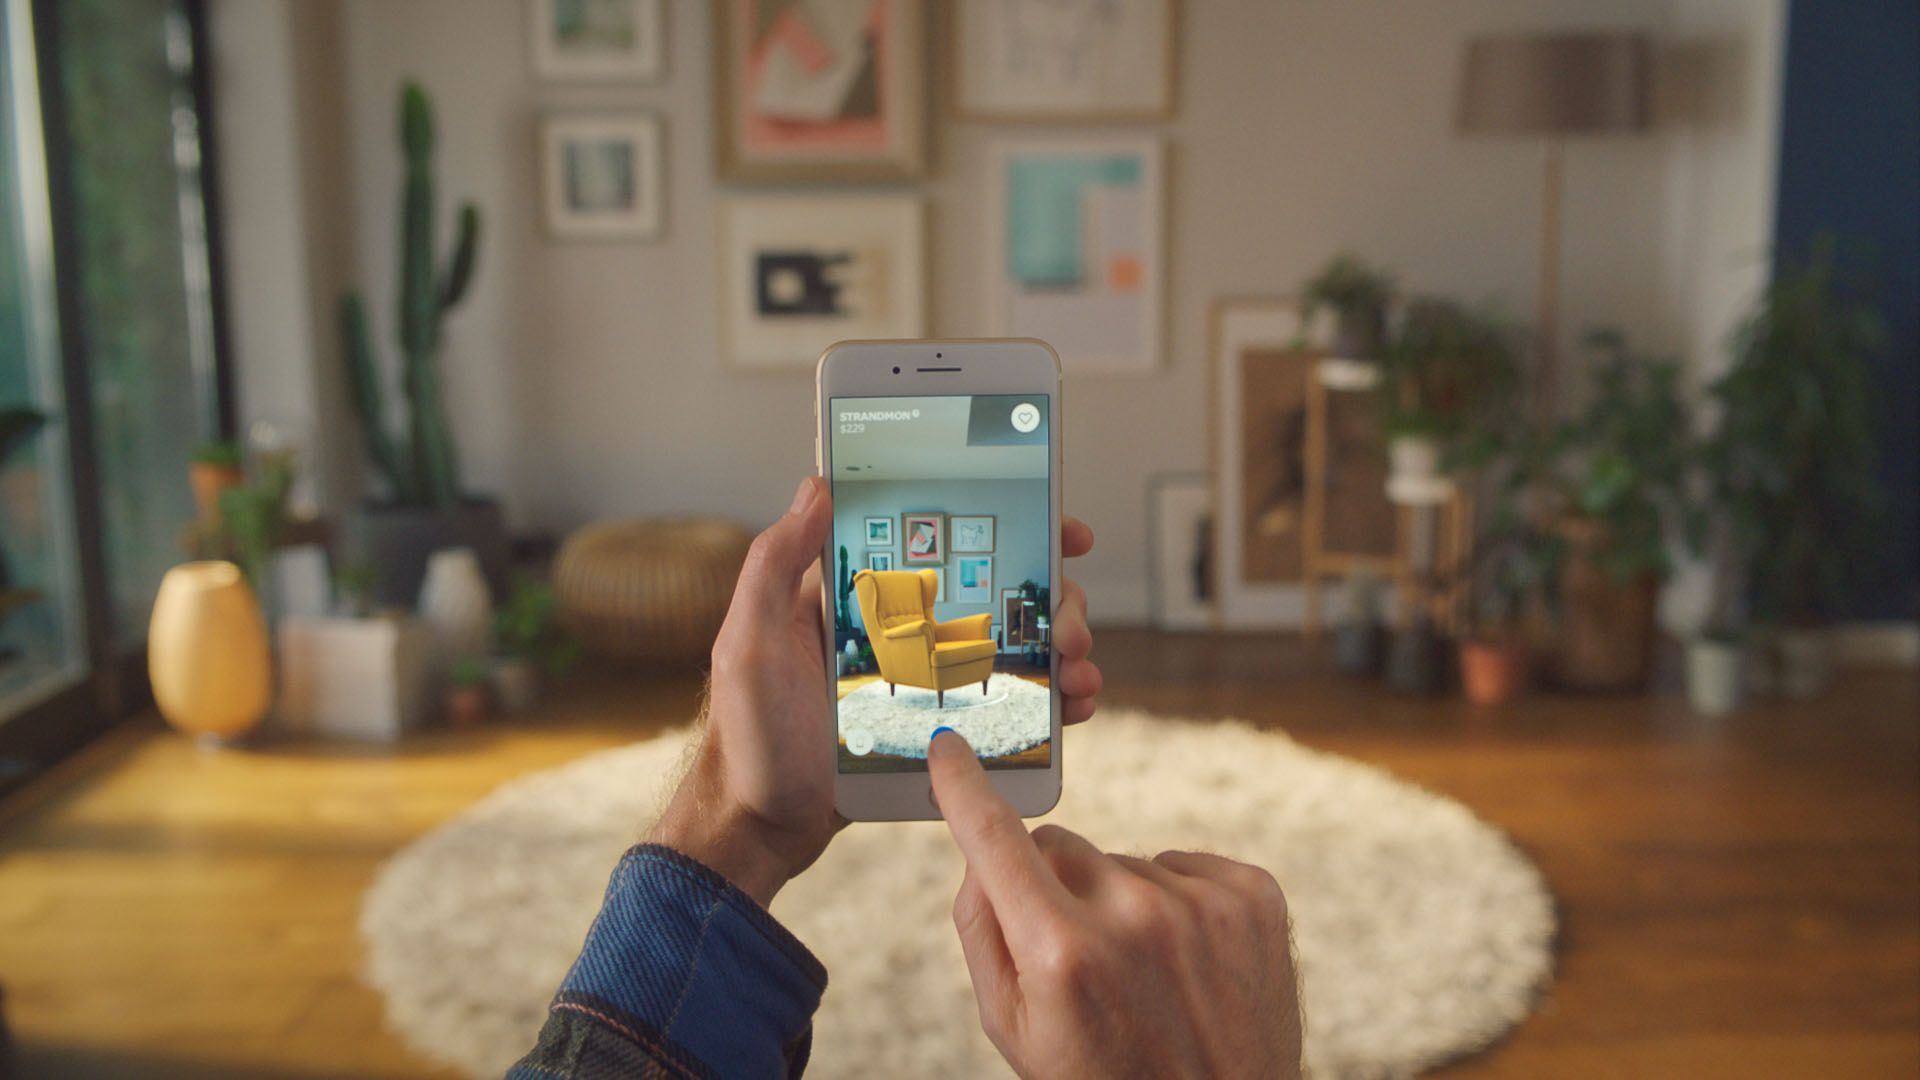
\includegraphics[scale=0.2]{images/ikea}
\end{center}
\pagebreak
\subsubsection{Rozšířená realita na základě projekce}
Tento přístup využívá projekci světla na povrchy v reálném světě k interakci s digitálními prvky. Senzory detekují změny v projekci a umožňují uživatelům reagovat na změny, což vytváří interaktivní zážitky. Tento typ pozicování je mnohem náročnější na výpočetní výkon, protože vyžaduje analýzu změn v projekcích a jejich korelaci s pohyby uživatele. \cite{AROverview} \\
Reálným příkladem rozšířené reality na základě projekce je interaktivní pískoviště. Poskytuje uživatelům možnost modelovat vlastní krajinu z písku a pozorovat, jak se v ní odehrávají různé přírodní procesy. \cite{IQLANDIAGeo} \\
\begin{center}
    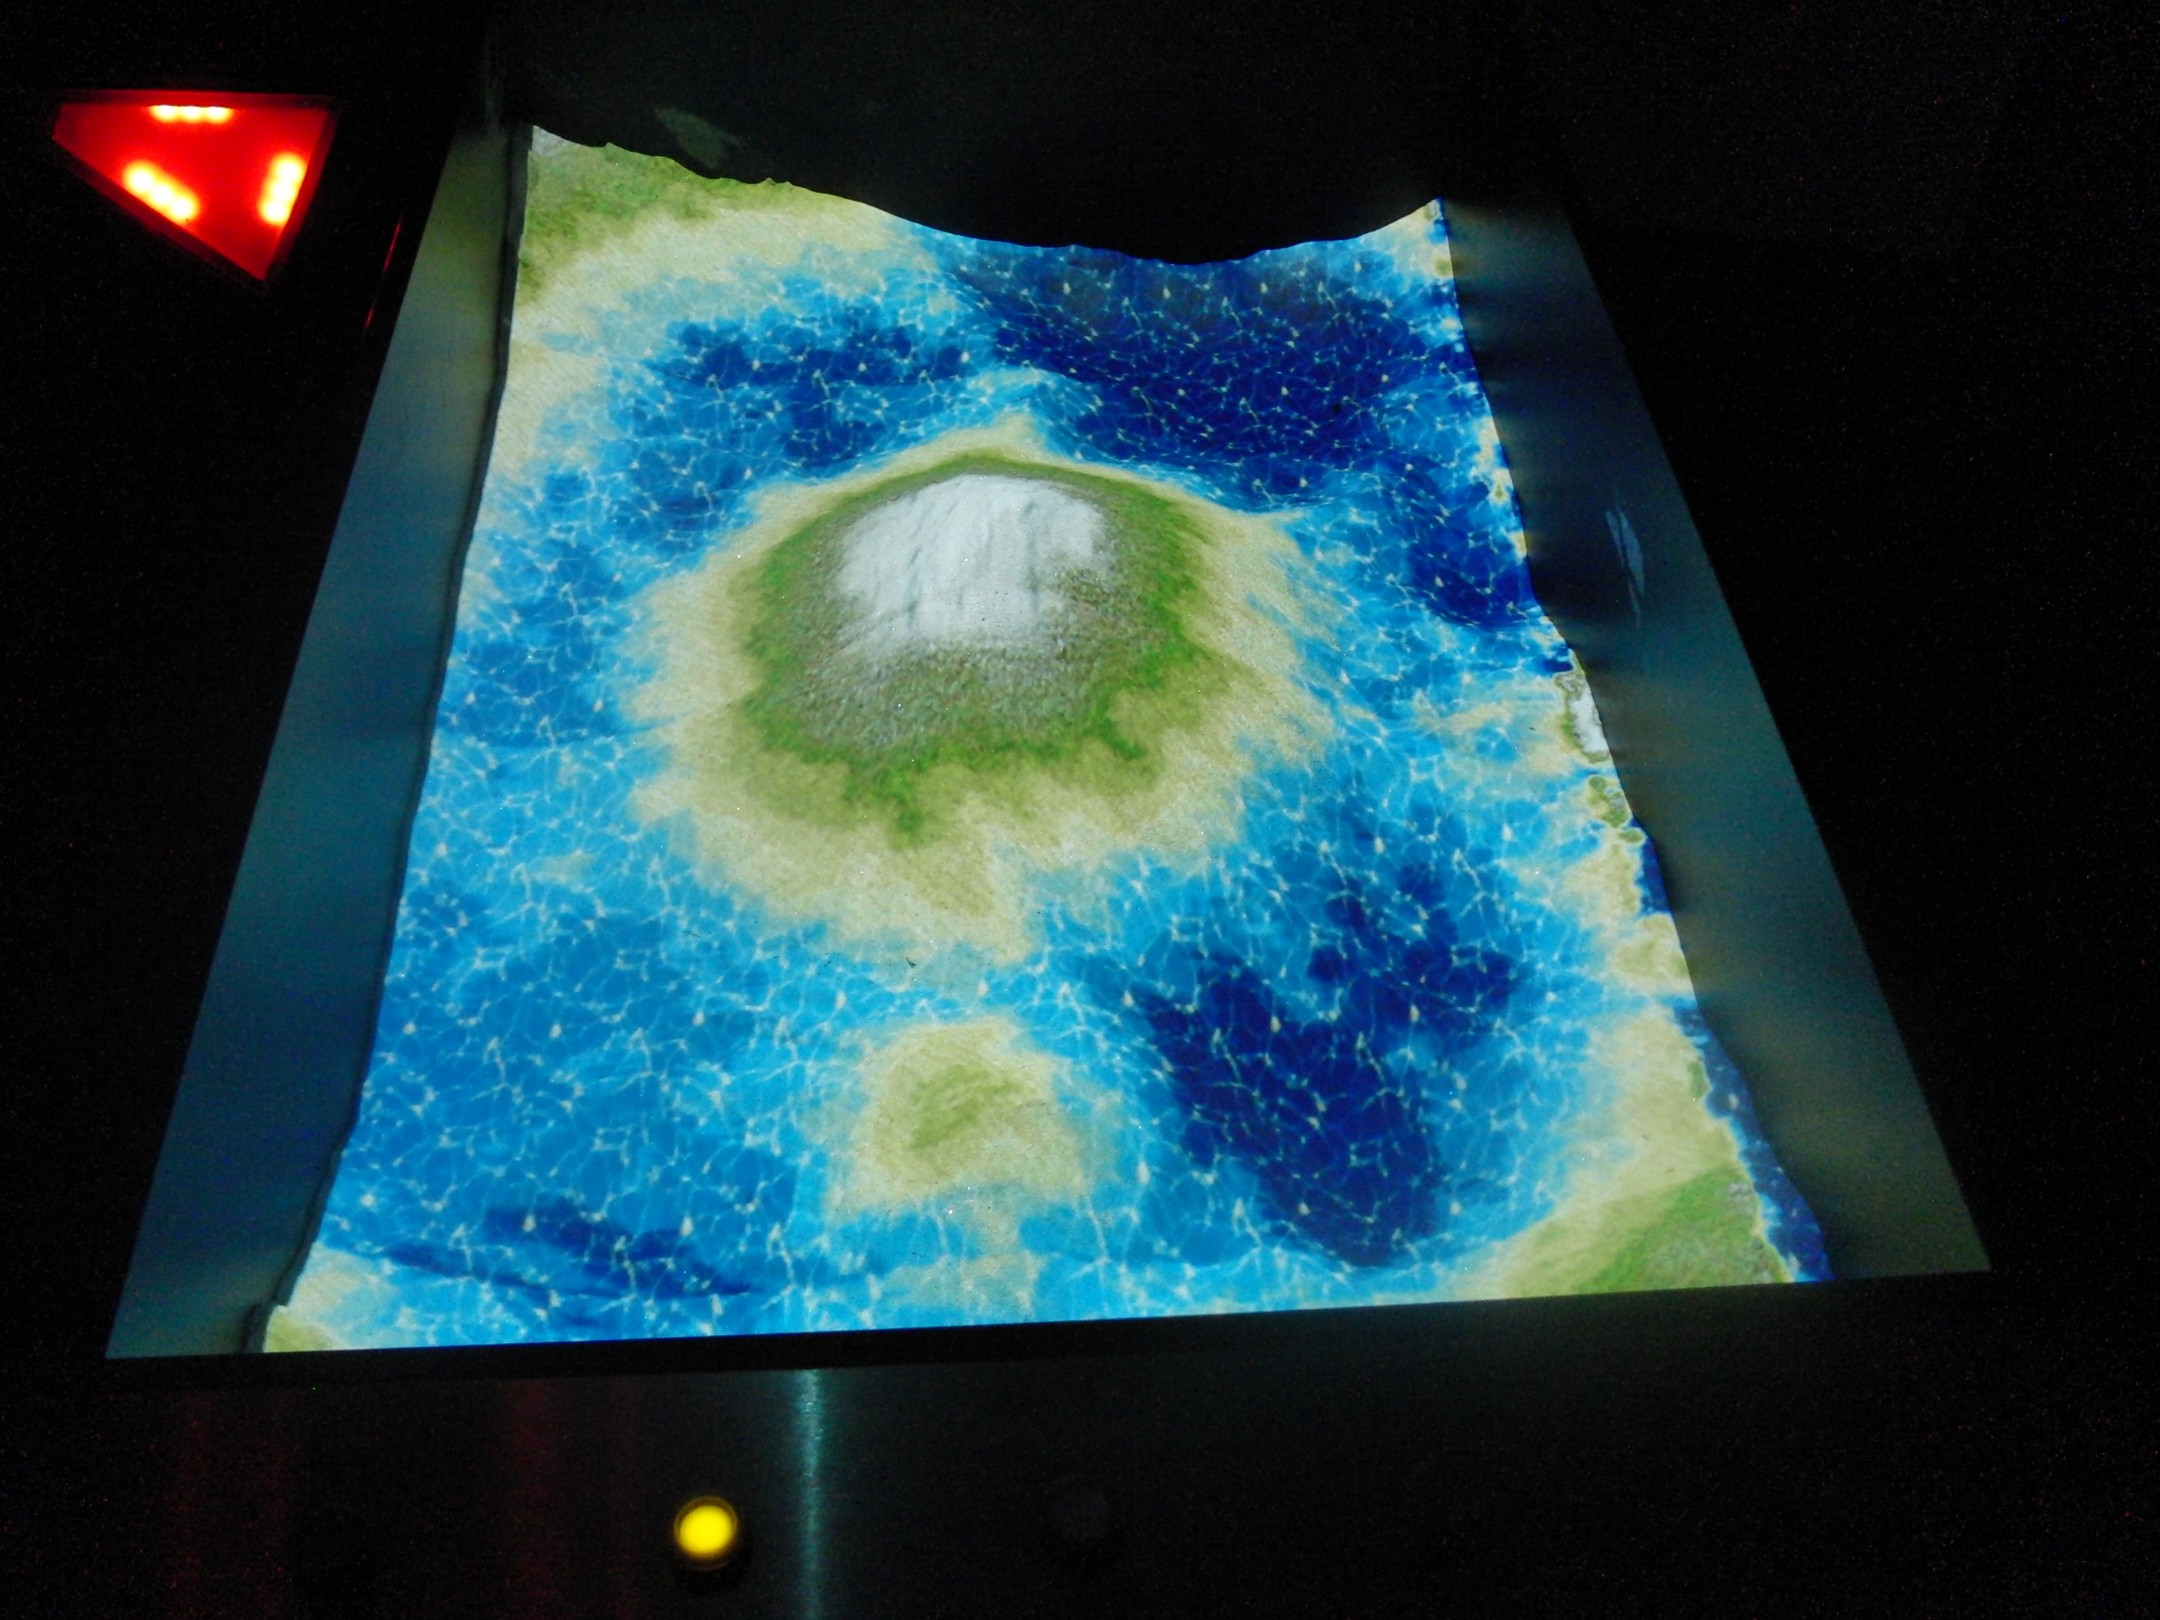
\includegraphics[scale=0.13]{images/IQLANDIA}
\end{center}
\subsubsection{Rozšířená realita pomocí překrytí}
Překrytí umožňuje úplné nebo částečné překrytí reálného objektu digitálními informacemi. U tohoto přístupu je klíčové rozpoznání objektů, protože aplikace musí správně identifikovat, kde se objekt nachází, aby ho mohla správně překrýt. \cite{AROverview} \\
Příkladem překrytí je Google Lens, již existující aplikace která poskytuje nástroje pro počítání příkladů, překlad textů a identifikaci předmětů prostřednictvím rozšířené reality. Pro lepší představu je obraz z kamery zpracován a následně dochází k překrytí reálného textu v cizím jazyce jeho překladem. \cite{googlelens}
\section{Přehled existujících řešení}